\documentclass{article}

\usepackage{graphicx}
\usepackage{amsmath}
\usepackage{fancyhdr}
\usepackage{float}
\usepackage{titlesec}
\usepackage{verbatim}
\usepackage{fancyvrb}
\usepackage[dvipsnames]{xcolor}
\usepackage[sorting=none]{biblatex}
\usepackage[margin=1in]{geometry}
\usepackage[font={small,it}]{caption}
\usepackage{placeins}
\usepackage{xepersian}


%%%%txt
\RecustomVerbatimCommand{\VerbatimInput}{VerbatimInput}%
{fontsize=\footnotesize,
 %
 frame=lines,  % top and bottom rule only
 framesep=2em, % separation between frame and text
 rulecolor=\color{Gray},
 %
 label=\fbox{\color{Black}txt file},
 labelposition=topline,
 %
 commandchars=\|\(\), % escape character and argument delimiters for
                      % commands within the verbatim
 commentchar=*        % comment character
}
%%%%txt


%\DeclareMathOperator*{\btie}{\bowtie}
\addbibresource{bibliography.bib}
\settextfont[Scale=1.2]{B-NAZANIN.TTF}
\setlatintextfont[Scale=1]{Times New Roman}
\renewcommand{\baselinestretch}{1.5}
\pagestyle{fancy}
\fancyhf{}
\rhead{تکلیف ششم آزمایشگاه شبکه ‌های کامپیوتری}
\lhead{\thepage}
\rfoot{علیرضا ابره فروش}
\lfoot{9816603}
\renewcommand{\headrulewidth}{1pt}
\renewcommand{\footrulewidth}{1pt}

\begin{document}
\begin{titlepage}
\begin{center}

\includegraphics[width=0.4\textwidth]{figures/IUT Logo.png}\\
        
\LARGE
\textbf{دانشگاه صنعتی اصفهان}\\
\textbf{دانشکده مهندسی برق و کامپیوتر}\\
        
\vfill
        
\huge
\textbf{عنوان: تکلیف چهارم درس ریزپردازنده}\\
        
\vfill
        
\LARGE
\textbf{نام و نام خانوادگی: علیرضا ابره فروش}\\
\textbf{شماره دانشجویی: 9816603}\\
\textbf{نیم\,سال تحصیلی: پاییز 1400}\\
\textbf{مدرّس: دکتر عارف کریمی افشار}\\
\end{center}
\end{titlepage}


%\tableofcontents
\newpage



\section{}%1
همانند جلسه قبل سناریو را می‌بندیم و روترها و \lr{PC}ها راپیکربندی می‌کنیم. توجه شود که تا مرحله‌ی 6 مراحل مثل جلسه قبل هستند. اما از مرحله‌ی 7 به بعد به جای مسیریابی استاتیک از پروتکل \lr{RIP} استفاده می‌کنیم.
\subsection{7}
در پروتکل \lr{RIP} برخلاف مسیریابی استاتیک، شبکه‌هایی که مستقیما به روتر وصل‌اند را پیکربندی می‌کنیم. برای پیکربندی پروتکل \lr{RIP} به شکل زیر عمل می‌کنیم.
\begin{figure}[H]
    \centering
    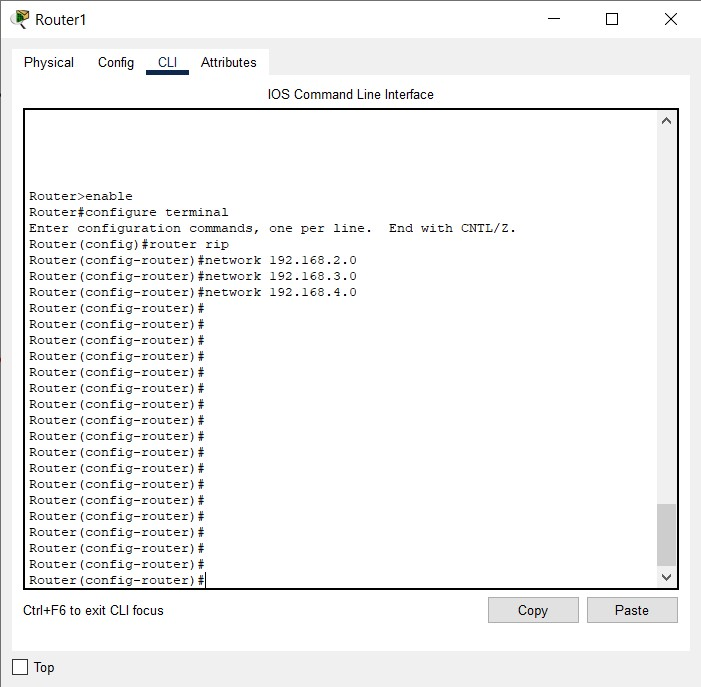
\includegraphics[width=0.75\textwidth]{figures/1.jpg}
    \caption{}
    \label{fig:fig1}
\end{figure}
به همین ترتیب برای سایر روترها شبکه‌هایی که مستقیما به آن‌ها متصل‌اند را پیکربندی می‌کنیم.


\subsection{8}
جداول مسیریابی روترها را در زیر می‌بینیم.
\begin{figure}[H]
    \centering
    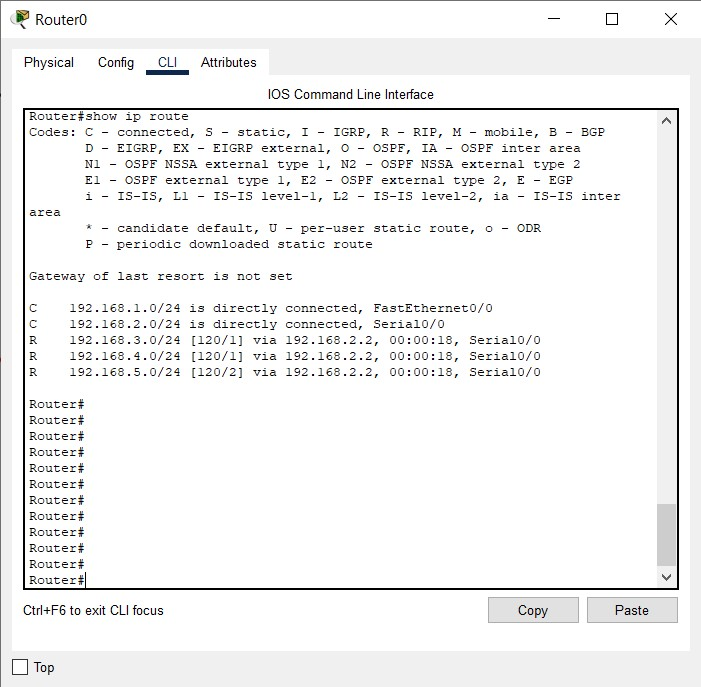
\includegraphics[width=0.75\textwidth]{figures/5.jpg}
    \caption{}
    \label{fig:fig1}
\end{figure}
\begin{figure}[H]
    \centering
    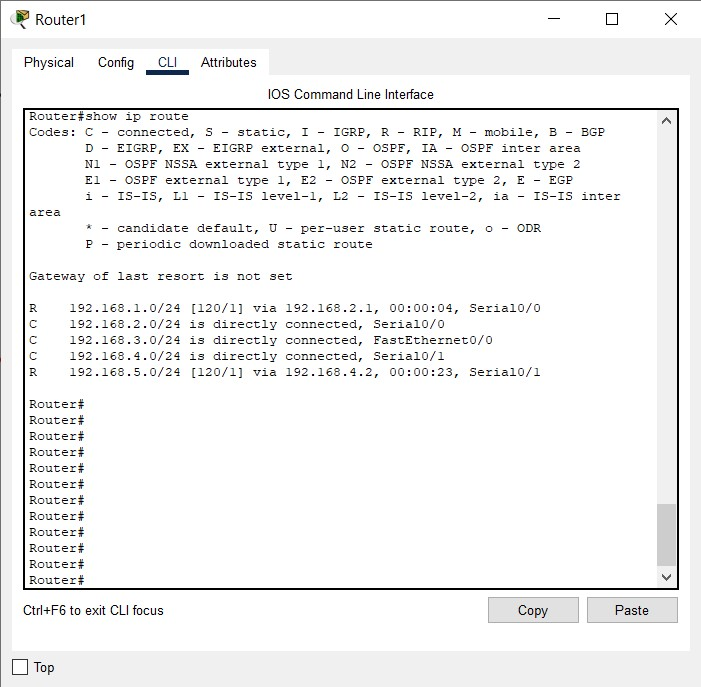
\includegraphics[width=0.75\textwidth]{figures/6.jpg}
    \caption{}
    \label{fig:fig1}
\end{figure}
\begin{figure}[H]
    \centering
    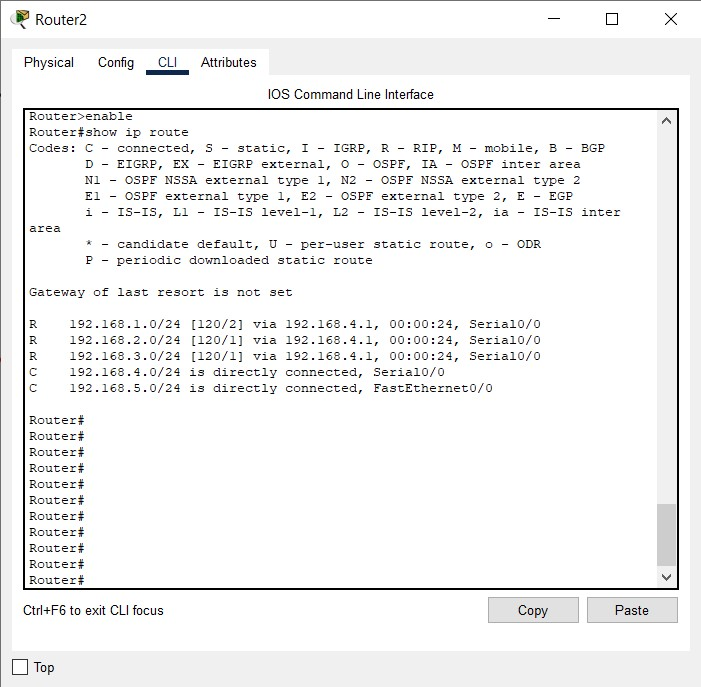
\includegraphics[width=0.75\textwidth]{figures/7.jpg}
    \caption{}
    \label{fig:fig1}
\end{figure}

\subsection{9}
جزئیات بیشتر از پروتکل \lr{RIP} تنظیم شده روی روتر‌ها را در زیر می‌بینیم.
\begin{figure}[H]
    \centering
    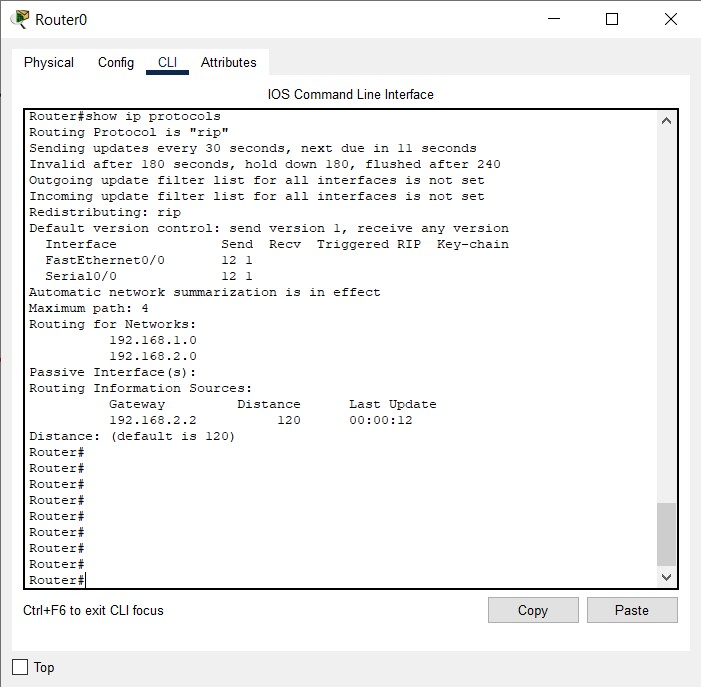
\includegraphics[width=0.75\textwidth]{figures/8.jpg}
    \caption{}
    \label{fig:fig1}
\end{figure}
\begin{figure}[H]
    \centering
    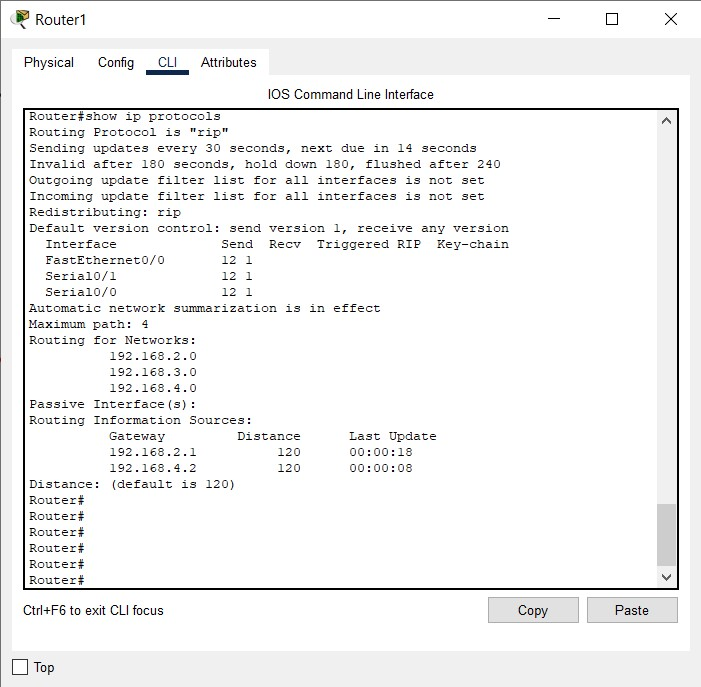
\includegraphics[width=0.75\textwidth]{figures/9.jpg}
    \caption{}
    \label{fig:fig1}
\end{figure}
\begin{figure}[H]
    \centering
    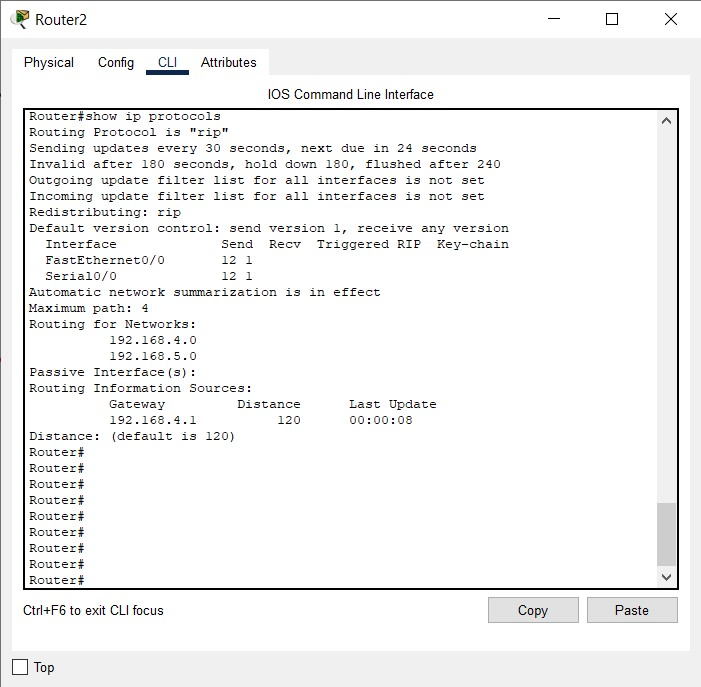
\includegraphics[width=0.75\textwidth]{figures/10.jpg}
    \caption{}
    \label{fig:fig1}
\end{figure}

\subsection{10}
همانطور که در تصاویر زیر می‌بینیم ارتباط بین تمام اجزای شبکه برقرار است.
\begin{figure}[H]
    \centering
    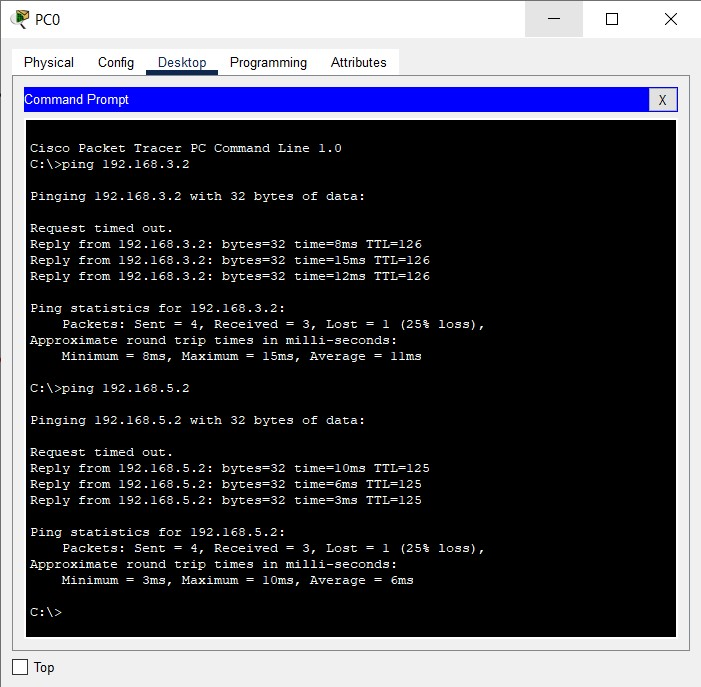
\includegraphics[width=0.75\textwidth]{figures/2.jpg}
    \caption{}
    \label{fig:fig1}
\end{figure}
\begin{figure}[H]
    \centering
    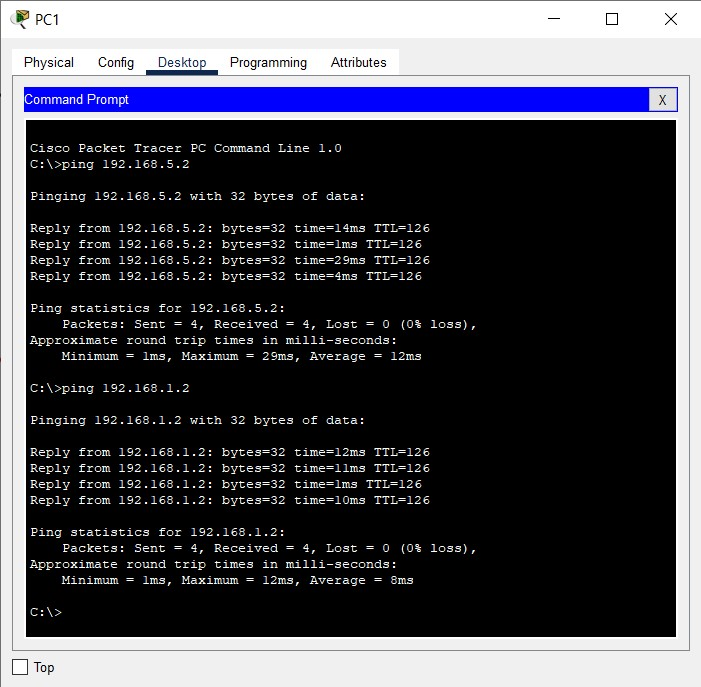
\includegraphics[width=0.75\textwidth]{figures/3.jpg}
    \caption{}
    \label{fig:fig1}
\end{figure}
\begin{figure}[H]
    \centering
    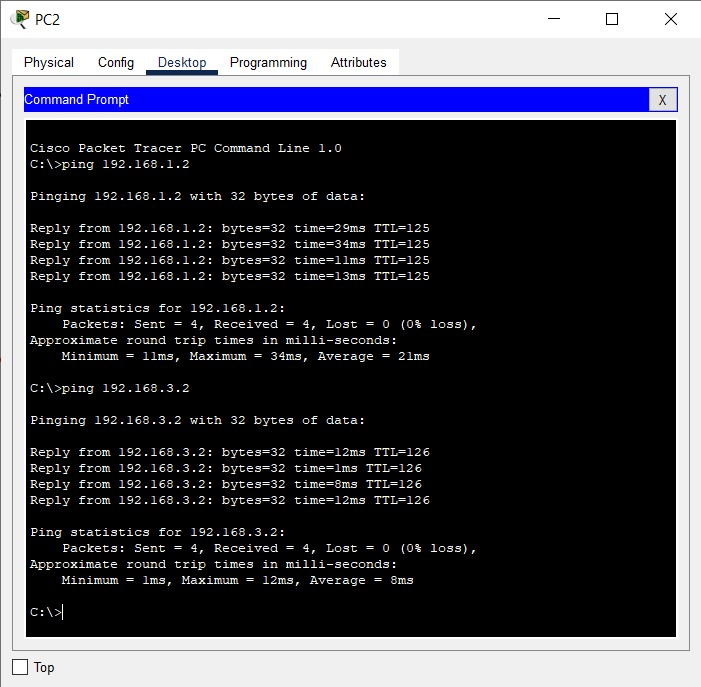
\includegraphics[width=0.75\textwidth]{figures/4.jpg}
    \caption{}
    \label{fig:fig1}
\end{figure}


\subsection{11}
\begin{figure}[H]
    \centering
    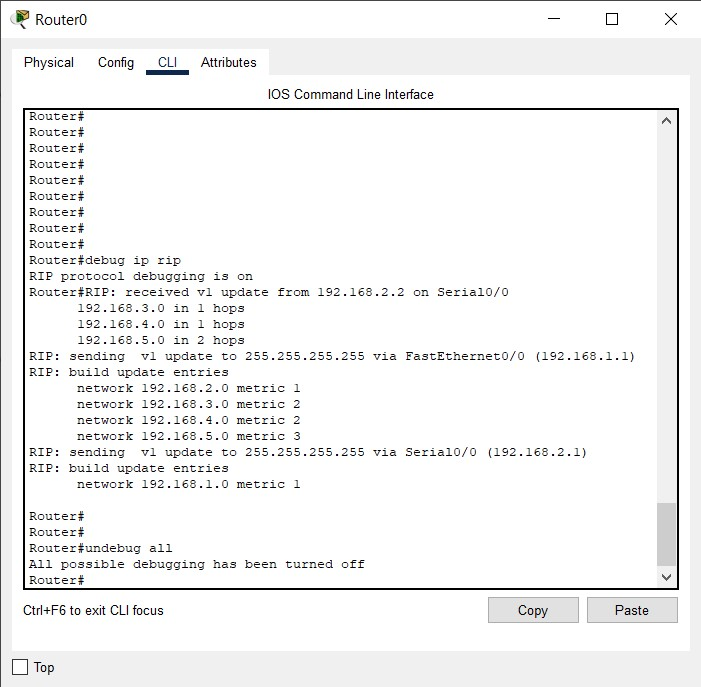
\includegraphics[width=0.75\textwidth]{figures/11.jpg}
    \caption{}
    \label{fig:fig1}
\end{figure}
\begin{figure}[H]
    \centering
    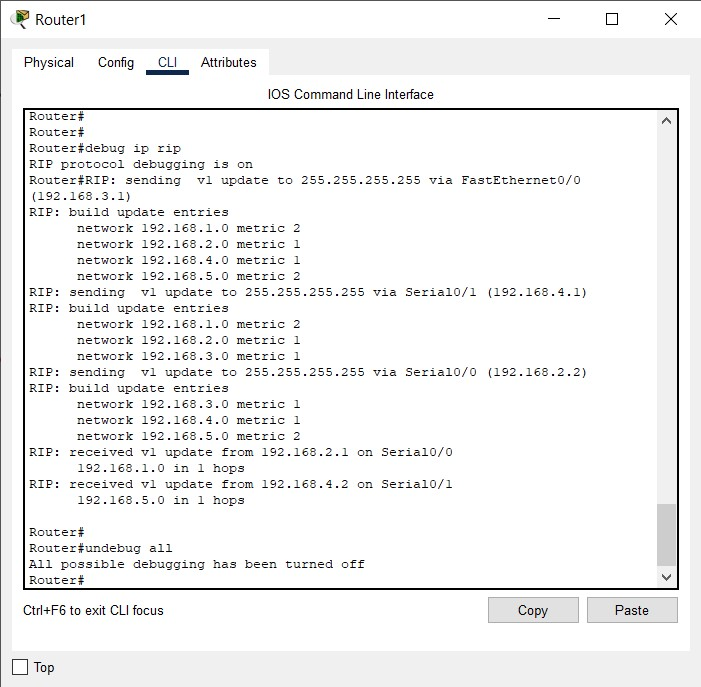
\includegraphics[width=0.75\textwidth]{figures/12.jpg}
    \caption{}
    \label{fig:fig1}
\end{figure}
\begin{figure}[H]
    \centering
    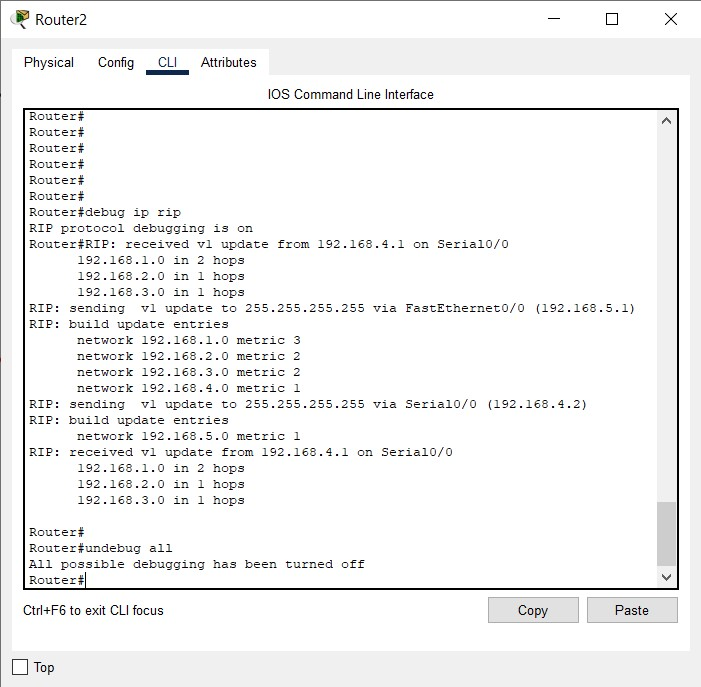
\includegraphics[width=0.75\textwidth]{figures/13.jpg}
    \caption{}
    \label{fig:fig1}
\end{figure}



\subsection{12}
خیر لزومی ندارد. هر روتر لازم است جدول مسیریابی خود را تنها به روترهای همسایه‎ی خود \lr{advertise} کند. پس فقط در اینترفیس‎های سریال لازم است که این جداول ارسال شوند. در صورتی که این \lr{advertisement}ها در شبکه‌های محلی که به هیچ روتر دیگری متصل نیستند رخ دهد باعث ایجاد بار ترافیکی بیهوده روی شبکه می‌شود.


\subsection{13 و 14}
خروجی دستور \lr{show ip protocols} قبل از اجرای دستور و پس از اجرای دستور را در زیر می‌بینیم.
\begin{figure}[H]
    \centering
    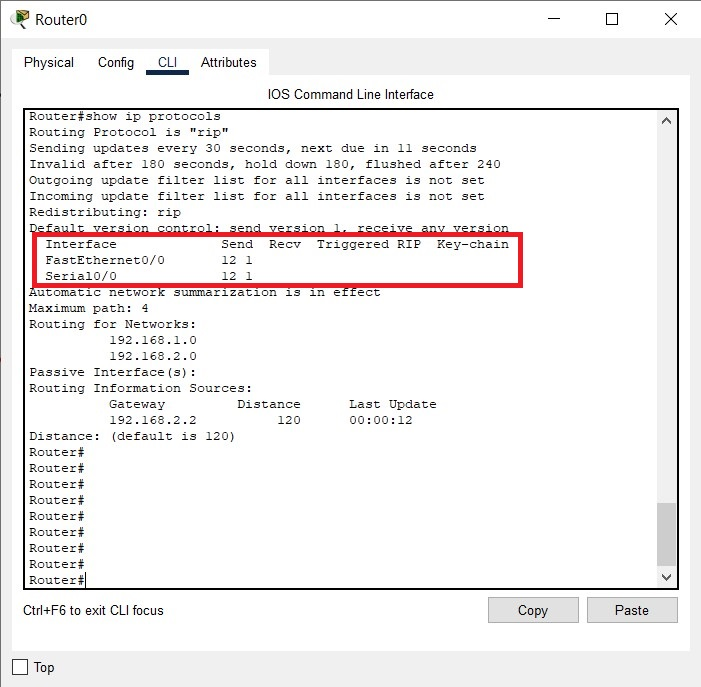
\includegraphics[width=0.75\textwidth]{figures/15.jpg}
    \caption{قبل از اجرای دستور}
    \label{fig:fig1}
\end{figure}
\begin{figure}[H]
    \centering
    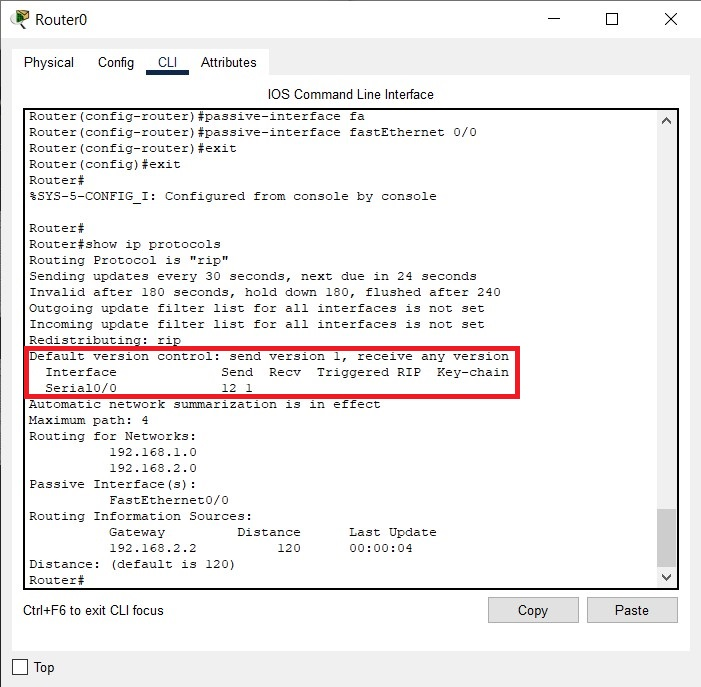
\includegraphics[width=0.75\textwidth]{figures/14.jpg}
    \caption{بعد از اجرای دستور}
    \label{fig:fig1}
\end{figure}




\section{}%2
\subsection{}
سناریوی جدید را به شکل زیر می‌بندیم.
\begin{figure}[H]
    \centering
    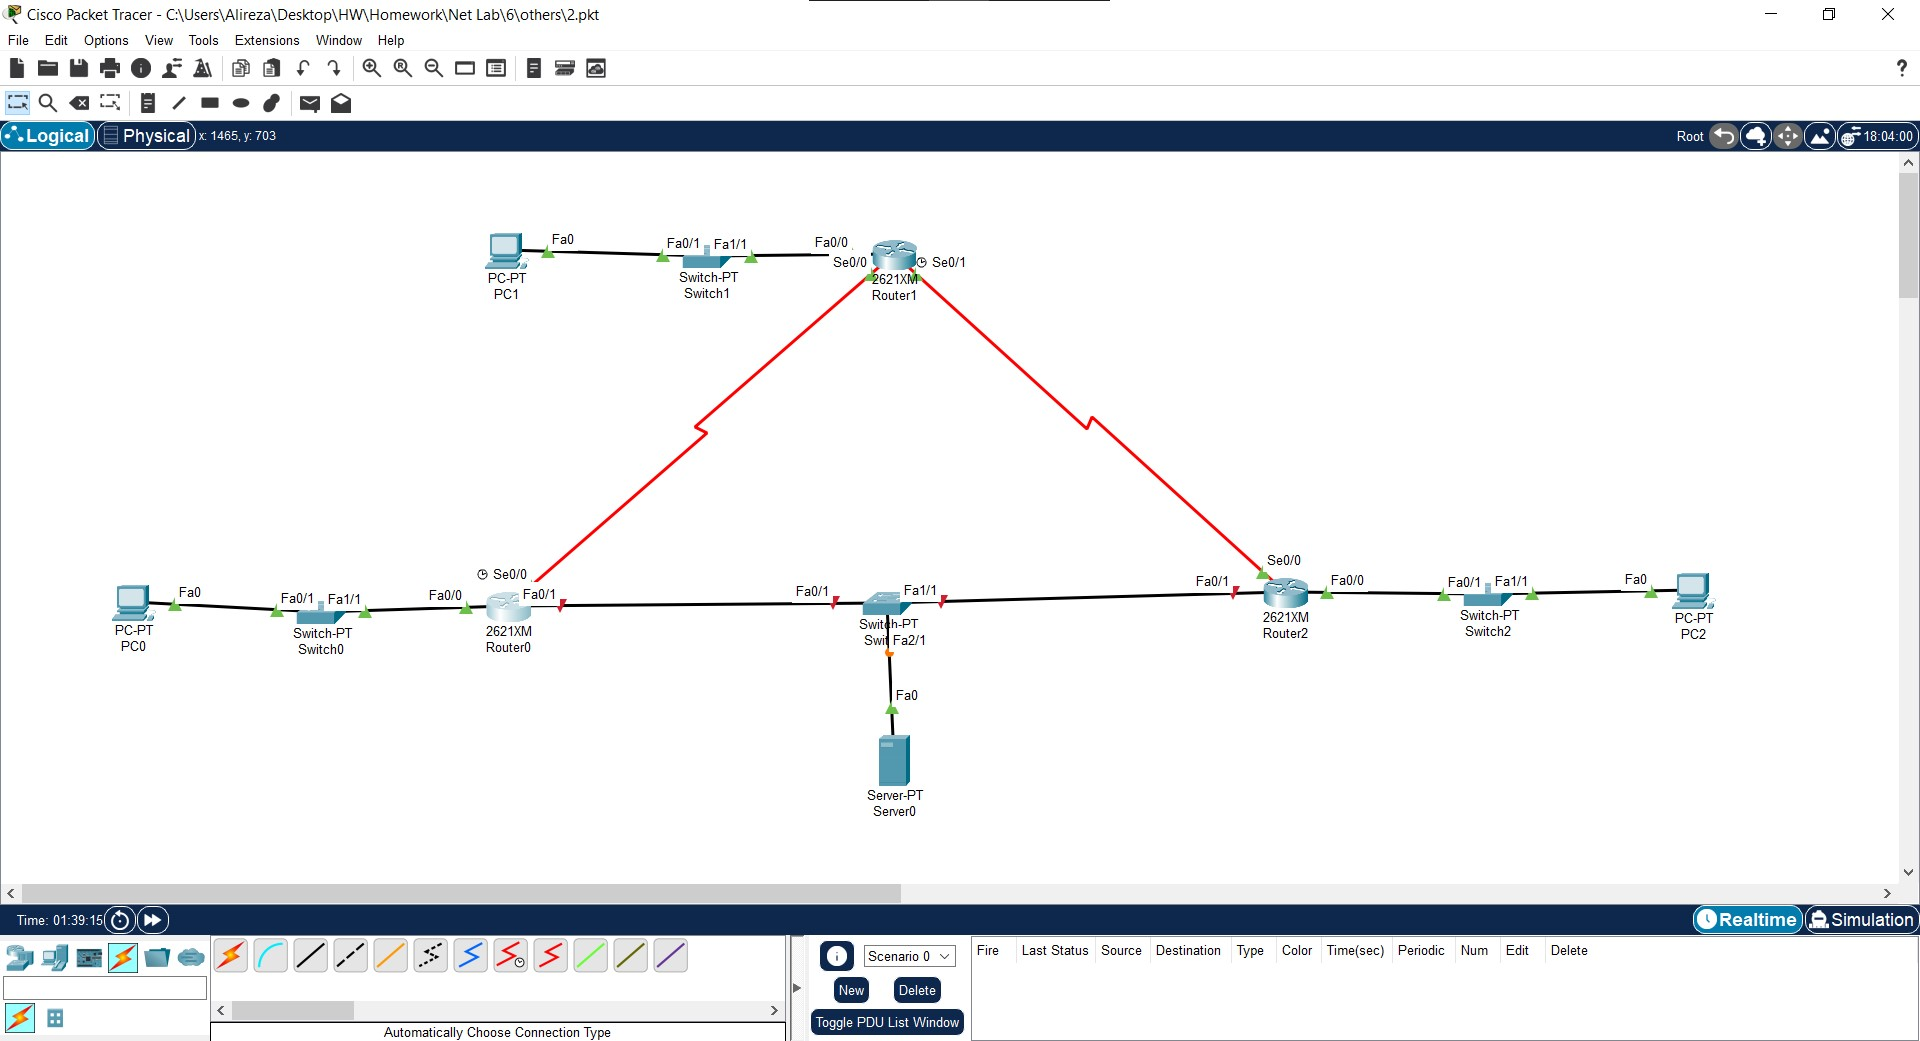
\includegraphics[width=1.0\textwidth]{figures/16.jpg}
    \caption{}
    \label{fig:fig1}
\end{figure}


\subsection{}
اینترفیس‌های جدید را به شکل زیر آدرس‌دهی می‌کنیم.
\begin{figure}[H]
    \centering
    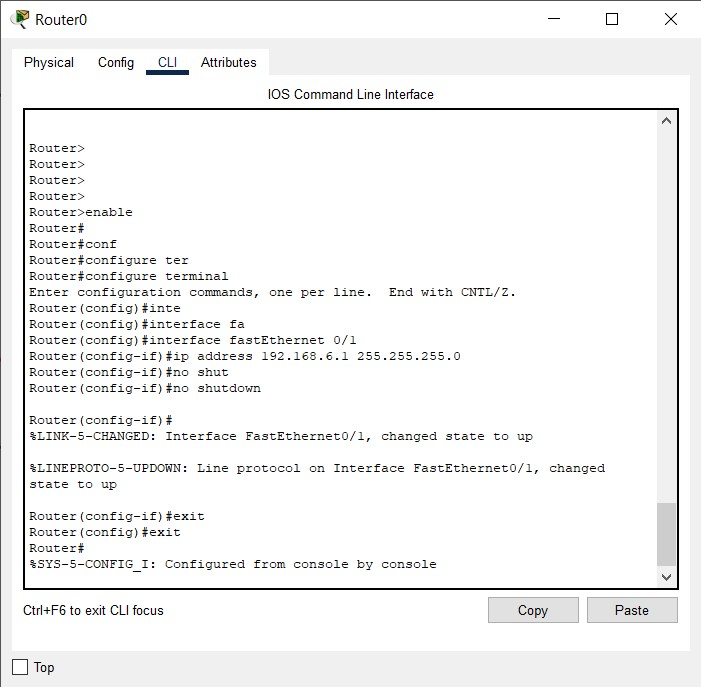
\includegraphics[width=0.75\textwidth]{figures/17.jpg}
    \caption{}
    \label{fig:fig1}
\end{figure}
\begin{figure}[H]
    \centering
    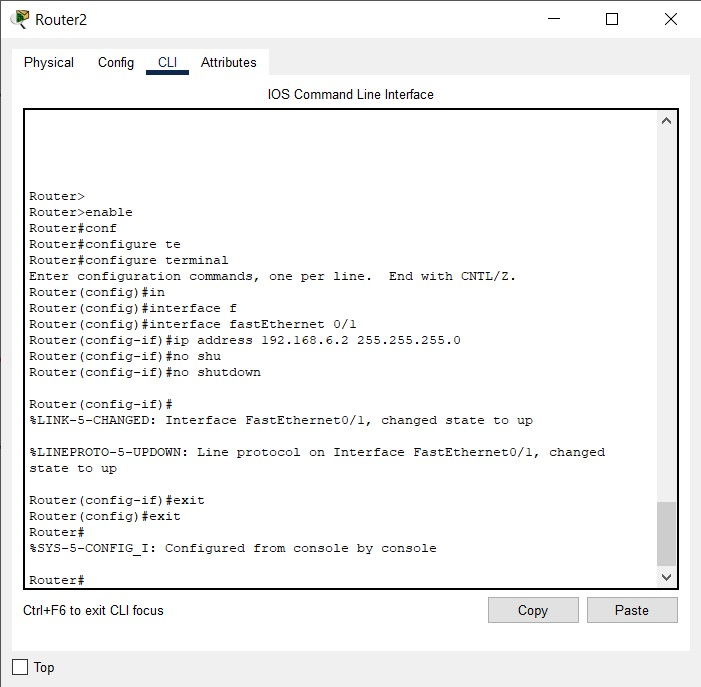
\includegraphics[width=0.75\textwidth]{figures/18.jpg}
    \caption{}
    \label{fig:fig1}
\end{figure}
\begin{figure}[H]
    \centering
    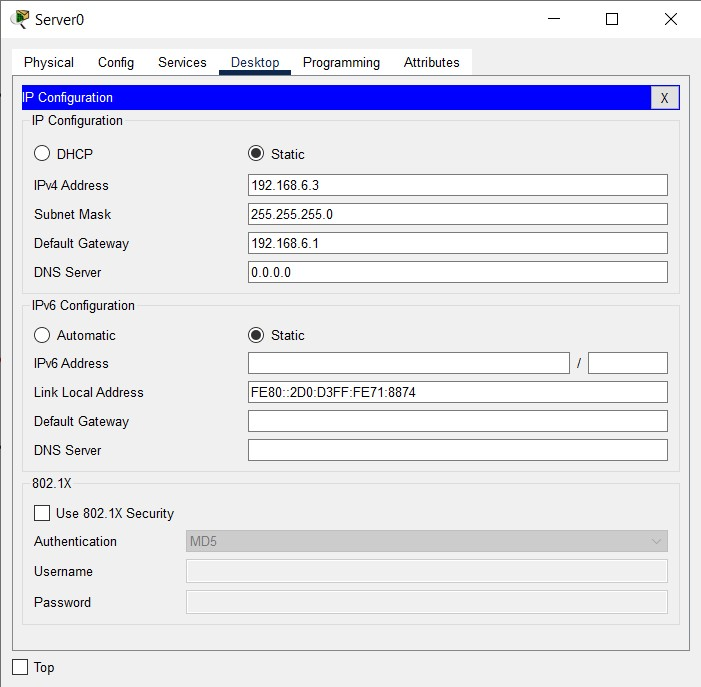
\includegraphics[width=0.75\textwidth]{figures/19.jpg}
    \caption{}
    \label{fig:fig1}
\end{figure}

\subsection{}
اینترفیس‌های جدید را به شکل زیر آدرس‌دهی می‌کنیم.
\begin{figure}[H]
    \centering
    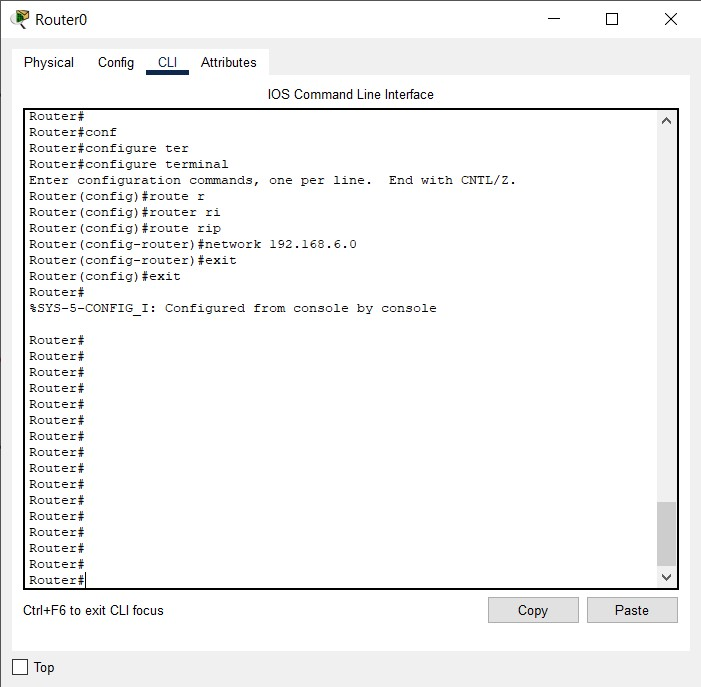
\includegraphics[width=0.75\textwidth]{figures/20.jpg}
    \caption{}
    \label{fig:fig1}
\end{figure}
\begin{figure}[H]
    \centering
    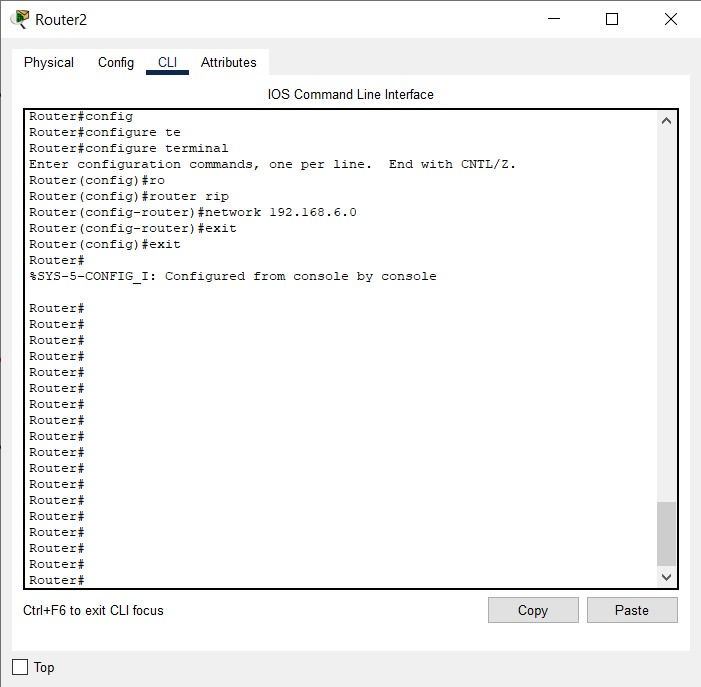
\includegraphics[width=0.75\textwidth]{figures/21.jpg}
    \caption{}
    \label{fig:fig1}
\end{figure}


\subsection{4 و 5}
از آنجایی که جدول مسیریابی روتر 0 به مقصد \lr{192.168.6.3} دارای دو \lr{entry}ِ  \lr{192.168.2.1} و  \lr{192.168.4.2} می‌باشد و مقدار \lr{AD} و تعداد \lr{HOP}ها در هر دو مسیر به ترتیب برابر 120 و 1 است، و از لحاظ هزینه هیچ کدام بر دیگری ارجحیت ندارد. اما احتمالا چون آدرس \lr{Gateway} سرور برابر \lr{192.168.6.1} است پکت‌ها از سمت \lr{192.168.2.1} به سرور هدایت می‌شوند.

\begin{figure}[H]
    \centering
    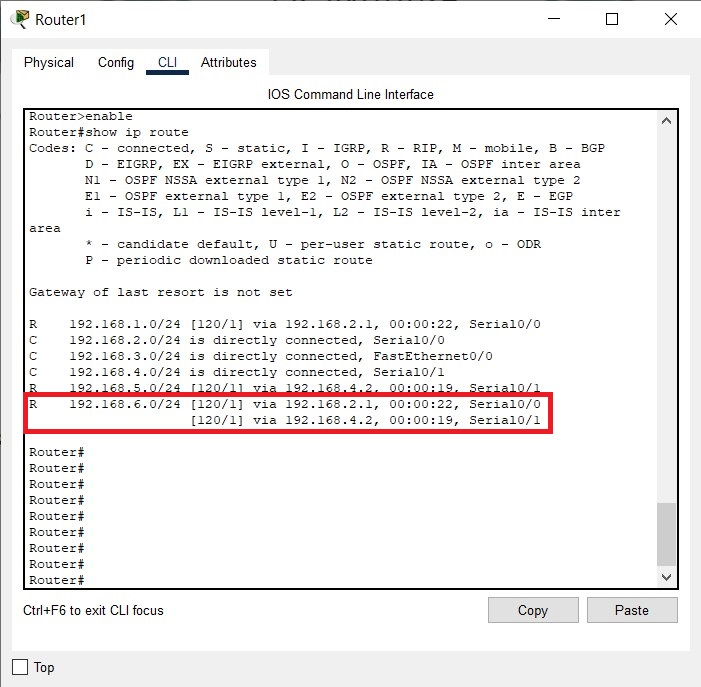
\includegraphics[width=0.75\textwidth]{figures/22.jpg}
    \caption{}
    \label{fig:fig1}
\end{figure}


\begin{figure}[H]
    \centering
    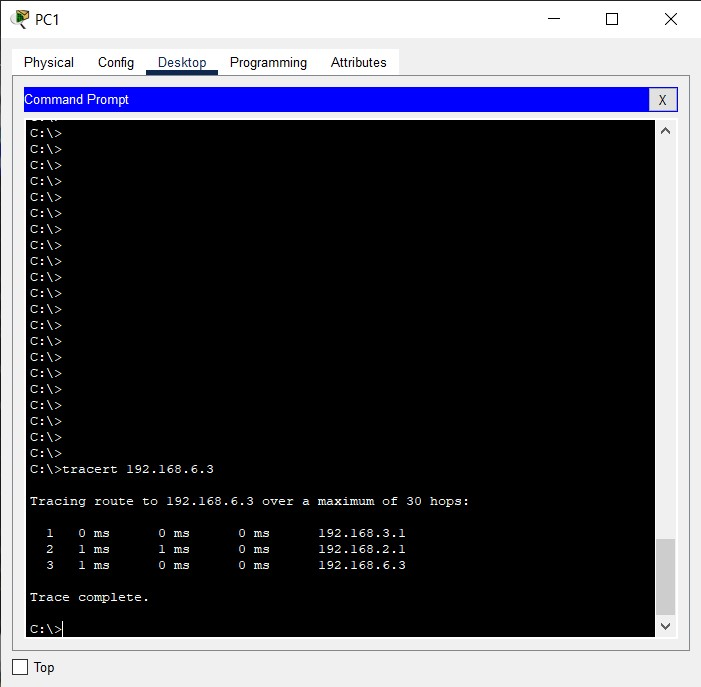
\includegraphics[width=0.75\textwidth]{figures/23.jpg}
    \caption{}
    \label{fig:fig1}
\end{figure}


%%%%%%%%%%%%%%%%%%%%%%%%%%%%%%%%%%%%%%%%%%%%%%

\section*{منابع}
\renewcommand{\section}[2]{}%
\begin{thebibliography}{99} % assumes less than 100 references
%چنانچه مرجع فارسی نیز داشته باشید باید دستور فوق را فعال کنید و مراجع فارسی خود را بعد از این دستور وارد کنید


\begin{LTRitems}

\resetlatinfont

\bibitem{b1}
\end{LTRitems}

\end{thebibliography}


\end{document}
